
Masinnägemise süsteemide loomiseks on olemas erinevaid tarkvaralisi lahendusi. Antud töö tarkvara hõlmab endas mitmeid üksteisest sõltuvaid osi: pilditöötlus ja edastamine, andmetöötlus ja närvivõrgud.

\textbf{Pilditöötluseks} on saadaval mitmeid mooduleid (OpenCV \cite{ref36}, Scikit-Image \cite{ref37}, SciPy \cite{ref38}, Pillow \cite{ref39}), mille hulgast masinõppe jaoks spetsiifiliselt on loodud OpenCV ja Scikit-Image. Antud ülesande lahendamisel rakendati OpenCV moodulit Scikit-Image asemel, kuna esimesel on ka olemas videote lugemise tugi Gstreameri \cite{ref40} näol, mis võimaldab kasutada Jetson arvutisse integreeritud Nvidia video dekoodrit \cite{ref41}. See säästab protsessorit pildivoo lugemisel ning teeb seda ka oluliselt efektiivsemalt, jättes pilditöötluse ning masinnägemise mudeli töö jaoks arvuti protsessorile rohkem võimekust alles.

\textbf{Andmetöötluse} jaoks on laialdasel kasutusel Pandas \cite{ref42} moodul, mis võimaldab lihtsate ning intuitiivsete käskudega andmeid analüüsida ning nendega manipuleerida. Antud moodul teeb toiminguid protsessori peal ning ekstreemsemate andmemahtude puhul võib andmete töötlemine ajamahukaks minna. Lisaks Pandasele on loodud mitmeid alternatiivseid mooduleid, mis on sarnaselt või minimaalse vahega paremini optimeeritud, kuid nendest kõige sarnasema tööpõhimõtte ja kirjakeelega on cuDF \cite{ref44}. CuDF on olemuselt kõige sarnasem Pandasega, kuid kasutab protsessori asemel graafikakaarti andmete töötluseks, mis just suurte andmemahtude talitlemisel annab ajaliselt suure eelise Pandase ees, kuna andmete töötlus toimub palju suurema paralleelsusega, kui protsessorit kasutades. Antud töö kirjutamise hetkel on kasutuses Pandase moodul, kuna töö autoril on selle mooduliga laialdasem töötamise kogemus ning. Hiljem on plaan minna üle cuDFiga arendamisele tarkvara optimeerimise eesmärkidel.

\textbf{Närvivõrkude} loomiseks on olemas mitmeid platvorme ning raamistikke: TensorFlow \cite{ref45}, Keras \cite{ref46}, PyTorch \cite{ref47}, Scikit-Learn \cite{ref48}, mille hulgast populaarseimad ning laialdasemas kasutuses on TensorFlow ja PyTorch. Antud töös kasutati PyTorchi, kuna võrreldes TensorFlowiga on PyTorchi süntaks rohkem püütonlik, mistõttu on ka seda Pythoni objektidega lihtsam ühildada ning veateadete puhul kergem aru saada kus viga tekkis. Samuti on töö autoril eelnev kogemus PyTorchiga arendamisel.

\section{Masinnägemise närvivõrgu mudel}\label{masinnuxe4gemise-nuxe4rvivuxf5rgu-mudel}

Objektide tuvastamiseks on saadaval mitmeid mudeleid, mis erinevad üksteisest täpsuse, sisendresolutsiooni, suuruse ja kiiruse poolest. Mudeli valimisel tuleb arvestada süsteemi jõudlusega, võimekamad süsteemid nagu näiteks serverid, suudavad jooksutada massiivseid ning täpseid mudeleid paralleelselt ja minimaalse mõjuga sisendite töötlemise kiirusele. Väiksemad süsteemid nagu sülearvutid ning manussüsteemid seevastu oleksid sobivamad väiksemate ning suurema kiirusega mudelite jooksutamiseks.

\begin{longtable}[]{@{}
  >{\raggedright\arraybackslash}p{0.2453\linewidth}
  >{\raggedright\arraybackslash}p{0.2830\linewidth}
  >{\raggedright\arraybackslash}p{0.2170\linewidth}
  >{\raggedright\arraybackslash}p{0.2358\linewidth}@{}}
\caption{Populaarseimate mudelite parameetrite ülevaade}\label{tab:4-1-1}\\
\toprule\noalign{}
\endhead
\bottomrule\noalign{}
\endlastfoot
\textbf{Mudel} & \textbf{Maksimaalne sisend (px)} & \textbf{Kiirus (ms)} & \textbf{Täpsus (mAP)} \\
FasterRCNN \cite{ref49} & 1000x600 & 198 & 73,2 (PASCAL VOC 2007) \\
YOLOv5 \cite{ref50} & 1280x1280 & 26,2 (V100 GPU) & 72,7 (MSCOCO) \\
MobileNet SSD V2 \cite{ref51} & 320x320 & 200 (Google Pixel 1) & 22,2 (MSCOCO) \\
EfficientDet \cite{ref52} & 1536x1536 & 153 (V100 GPU) & 55,1 (MSCOCO) \\
\end{longtable}

Antud süsteemi jaoks tuli mudeli valimisel arvestada parima mudeli täpsuse ja kiiruse suhtega. Samuti pidi valitav mudel olema ka võimeline mitmelt videosisendilt korraga infot töötlema (vt Tabel~\ref{tab:4-1-1}).

Antud ülesande lahendamiseks osutus valituks Yolov5 arhitektuuriga närvivõrk, mis on Ultralytics'i \cite{ref53} poolt loodud edasiarendusena Yolov4st \cite{ref54} ning on kiirem ja täpsem kui selle eelkäijad. Samuti on tegemist ka kompaktse mudeliga, mis on hõlpsasti sardsüsteemidel jooksutatav. Mudel toimib ühekordsel kaadri töötlemise filosoofial (\emph{You Only Look Once}) ehk pilt läbib võrku ainult ühe korra (erinevalt teistest mudelitest), mille käigus toimub objektituvastus ja klassifikatsioon korraga, mistõttu on ka mudeli tuvastuste operatsiooni kiirus suurem (vt Joonis~\ref{fig:image12}).

\begin{figure}[H]
\centering
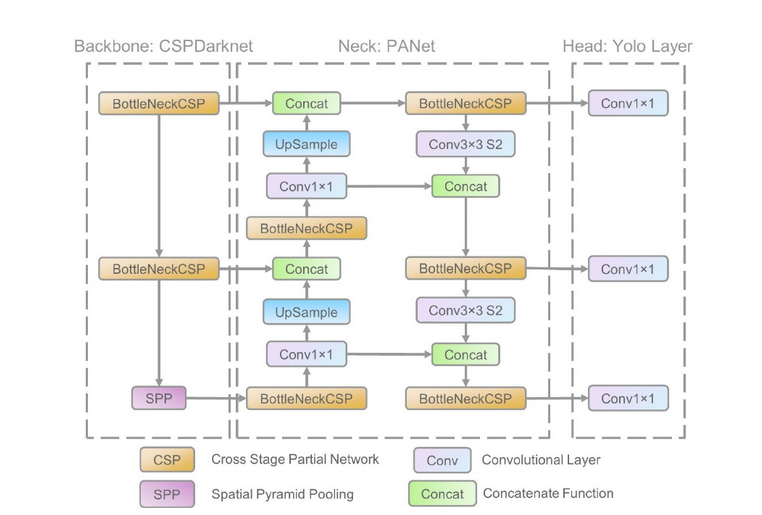
\includegraphics[width=6.10174in,height=4.125in]{media/image12.png}
\caption{Yolov5 mudelite arhitektuur \cite{ref55}}\label{fig:image12}
\end{figure}

Mudel koosneb kolmest osast: Selgroog, kael ja pea.

\begin{itemize}
\item
  \textbf{Selgroog} (\emph{backbone}) ehk baas millele mudel ehitatakse, antud juhul on selleks valitud CSPNet (\emph{Cross-Stage Partial Network}). Tegemist on närvivõrgu mudeli tüübiga, mis on jaotatud mitmeks osaks (\emph{Cross-Stage}), milles iga kiht tegeleb ette antud pildilt informatsiooni eraldamisega nagu äärised ja kujundid, mis on iseloomulikud antud objektile pildil. Osa informatsioonist mida eelnevates kihtides omastatakse, antakse edasi järgmistele kihtidele töötlemiseks (\emph{Partial}), mis võimaldab võrgul järgemööda paremini ning täpsemini aru saada mida pildil kujutatakse kasutades eelmistelt kihtidelt saadud töödeldud infot. Backbone koosneb peamiselt konvolutsioonilistest kihtidest ja allaskaleerimise kihist, mille väljund läheb edasi mudeli kaela. Taolise arhitektuuriga mudel aitab vähendada vajalike arvutuslike protsesside hulka.
\item
  \textbf{Kael} (\emph{neck}) närvivõrgus tegeleb selgroost saadud informatsiooni kokkupaneku ja organiseerimisega tunnusjoonte maatriksisse (\emph{feature map}), kasutades filtreid. Antud mudel rakendab ruumilist tähelepanu koondamise meetodit, mis aitab närvivõrgul keskenduda olulistele osadele pildil ja ruumilist püramiid-skaleerimise kihti (\emph{Spatial Pyramid Pooling}), mis võimaldab objekte tuvastada erinevatel resolutsioonidel.
\item
  \textbf{Pea} (\emph{head}) tegeleb tuvastuste tõenäosuste ning koordinaatide loomisega kaadrilt leitud objektidele. Antud mudelis kasutatakse ka ankurdamiskaste (\emph{anchor boxes}), mis on eelnevalt seadistatud kuvasuhetega, mis aitavad erinevate suurustega ning kujudega objekte tuvastada. Mudeli pea sisaldab endas hulka konvolutsioonilisi kihte, mis tegelevad tuvastuste koordinaatide ja tõenäosuste ennustamisega iga objekti kohta \cite{ref55}
\end{itemize}
